\documentclass[12p,a4paper]{article}

\usepackage[serbian]{babel} 
\usepackage[T2A]{fontenc} 
\usepackage[utf8]{inputenc} 
\usepackage{amsthm}
\usepackage{multicol} 
\usepackage[margin=0.5in]{geometry} 
\usepackage{amsmath} 
\usepackage{amsfonts} 
\usepackage{enumerate} 
\usepackage{amssymb}
\usepackage{tikz}
\usepackage{booktabs} 
\usepackage{graphicx} 
\usepackage{listings} 

\DeclareMathOperator{\Dom}{Dom} 
\DeclareMathOperator{\Ima}{Im} 
\DeclareMathOperator{\nzd}{NZD} 
\DeclareMathOperator{\nzs}{NZS} 
\DeclareMathOperator{\NOR}{NOR} 

\newtheorem*{theorem}{Teorema}
\newtheorem*{prop}{Tvrđenje}

\lstset{language=C}

\title{Uvod u Organizaciju i Arhitekturu Racunara 2 --- Cheat Sheet}
\author{Andrija Urošević}

\begin{document}

\maketitle

\begin{multicols}{2}

\section{Bulova Algebra}

    \subsection{Tabele Istinitosti}

    \begin{tabular}{*{8}{c}}
        A & B & AND & NAND & OR & NOR & NOT & XOR \\
        \midrule
        0 & 0 & 0 & 1 & 0 & 1 & 1 & 0 \\
        0 & 1 & 0 & 1 & 1 & 0 & 1 & 1 \\
        1 & 0 & 0 & 1 & 1 & 0 & 0 & 1 \\
        1 & 1 & 1 & 0 & 1 & 0 & 0 & 0 \\
    \end{tabular}

    \subsection{Osnovni Zakoni Bulove Algebre}

    \begin{itemize}
        \itemsep0em
        \item $x \cdot x = x, x + x = x$ (zakon idempotencije)
        \item $x \cdot 1 = x, x + 0 = x$ (zakon neutrala)
        \item $x \cdot (x + y) = x, x + x \cdot y$ (zakon apsorpcije)
        \item $\overline{\overline{x}} = x$ (zakon dvojne negacije)
        \item $\overline{x + y} = \overline{x} \cdot \overline{y},
            \overline{x \cdot y} = \overline{x} + \overline{y}$
            (De-Morganovi zakoni)
    \end{itemize}

    \subsection{Logicki Izrazi i Normalne Forme}

    Pridruzivanje 0 i 1 logickim promenljivima naziva se \emph{valuacija}, tj.
    \emph{valuacija} je bilo koje preslikavanje iz skupa promenljivih $P$ u 
    $\{0, 1\}$, $v: P \mapsto \{0, 1\}$. Ovakvih funkcija ima $2^{|P|}$

    Za dva logicka izraza $E_1, E_2$ kazemo da su \emph{ekvivalentni} ako 
    imaju jednake vrednosti u svakoj valuaciji.

    \subsubsection{Konjunktivna i Disjunktivna Normalna Forma}

    \emph{Literal} je logicka izraz koji se sastoji od logickih promenljivih 
    i njihovig negacija ($x, \overline{y}, z$).
    
    \emph{Elementarna konjunkcija} --- $\mathcal{EK}$ je logicki izraz koji se 
    sastoji od konjunkcije literala ($x \overline{y} z$).

    \emph{Elementarna disjunkcija} --- $\mathcal{ED}$ je logicki izraz koji se
    sastoji od disjunkcija literala ($ x + \overline{y} + z$).

    \emph{Disjunktivna normalna forma} --- $\mathcal{DNF}$ se sastoji od 
    disjunkcija elementarnih konjunkcija 
    ($x \overline{y} + \overline{x} y z + x z$).

    \emph{Konjunktivna normalna forma} --- $\mathcal{KNF}$ se sastoji od 
    konjunkcija elementarnih disjunkcija
    ($(x + \overline{y} ) \cdot (\overline{x} + y + z) \cdot (x + z)$).

    Algoritam svodjenja izraza $E$ na izraz $E'$ u $\mathcal{DNF}$:
    \begin{enumerate}
        \itemsep0em
        \item Eliminacija logickih konstanti 0 i 1.
        \item Eliminacija negacija na vise od jedne promenljive pomocu 
              De-Morganovih zakona.
        \item Primena distributivnosti.
    \end{enumerate}

    \subsubsection{Savrsena Konjunktivna i Disjunktivna Normalna Forma}

    Za $\mathcal{EK}$ kazemo da je \emph{savrsena} u odnosu na dati skup
    promenljivih $P$ ako sadrzi tacno po jedan literal za svako od 
    promenljivih iz $P$ ($P = \{x, y, z\}, x \overline{y} z$).

    Za $\mathcal{ED}$ kazemo da je \emph{savrsena} u odnosu na dati skup 
    promenljivih $P$ ako sadrzi tacno po jedan literal za svaku od
    prmenljivih iz $P$ ($P = \{x, y, z\}, x + \overline{y} + z$).

    Za $\mathcal{KNF}$ kazemo da je \emph{savrsen} ako su njegove 
    $\mathcal{ED}$ savrsene ($(x + y) (\overline{x} + y)$).

    Za $\mathcal{DNF}$ kazemo da je \emph{savrsen} ako su njegove 
    $\mathcal{EK}$ savrsene ($xy + \overline{x}y$).

    \subsection{Logicke Funkcije}
    
    \emph{Logicka funkcija reda $n$} je bilo koje preslikavanje
    $f: {\{0, 1\}}^n \mapsto \{0, 1\}$, koje svakoj $n$-torci logickih 
    vrednosti $(x_1, x_2, \ldots, x_n) \in {\{0, 1\}}^n$ pridruzuje vrednost
    $y = \{0, 1\}$, tj. $f(x_1, x_2, \ldots, x_n) = y$.

    Domen funkcije $f$ ima $2^n$ vrednosti, dok kodomen ima $2$ vrednosti. 
    Sledi da funkcija ima ukupna $2^{2^n}$ preslikavanja.

    Funkcije reda 1:

    \begin{tabular}{*{2}{c}}
        Ime funkcije        & Vrednost funkcije \\
        \midrule
        Nula funkcija       & $f(x) = 0$ \\
        Jedinicna funkcija  & $f(x) = 1$ \\
        Funkcija identiteta & $f(x) = x$ \\
        Funkcija negacije   & $f(x) = \overline{x}$ \\
    \end{tabular}

    Funkcije reda 2:

    \begin{tabular}{*{2}{c}}
        Ime funkcije                                    & Vrednost funkcije \\
        \midrule
        Nula funkcija                                   & $f(x, y) = 0$ \\
        Jedinicna funkcija                              & $f(x, y) = 1$ \\
        Prva projekcija                                 & $f(x, y) = x$ \\
        Druga projekcija                                & $f(x, y) = y$ \\
        Negacija prve projekcije                        & $f(x, y) = \overline{x}$ \\
        Negacija druge projekcije                       & $f(x, y) = \overline{y}$ \\
        Konjunkcija                                     & $f(x, y) = x y$ \\
        Disjunkcija                                     & $f(x, y) = x + y$ \\
        Seferova funkcija (NAND)                        & $f(x, y) = \overline{xy} = \overline{x} + \overline{y}$ \\
        Pirsova funkcija (NOR)                          & $f(x, y) = \overline{x + y} = \overline{x} \ \overline{y}$ \\
        Implikacija $x \implies y$                      & $f(x, y) = \overline{x} + y$ \\
        Implikacija $y \implies x$                      & $f(x, y) = \overline{y} + x$ \\
        Negacija implikacija $\overline{x \implies y}$  & $f(x, y) = x \overline{y}$ \\
        Negacija implikacija $\overline{y \implies x}$  & $f(x, y) = \overline{x} y$ \\
        Ekskluzivna disjunkcija $y \oplus x$            & $f(x, y) = x \overline{y} + \overline{x} y$ \\
        Ekvivalencija                                   & $f(x, y) = x y + \overline{x} \ \overline{y}$ \\
    \end{tabular}

    \subsubsection{Savrsena Disjunktivna/Konjunktivna Normalna Forma}

    \begin{tabular}{*{4}{c}}
        $x$ & $y$ & $z$ & $f(x, y, z)$ \\
        \midrule
        0 & 0 & 0 & 1 \\
        0 & 0 & 1 & 0 \\
        0 & 1 & 0 & 0 \\
        0 & 1 & 1 & 1 \\
        1 & 0 & 0 & 0 \\
        1 & 0 & 1 & 1 \\
        1 & 1 & 0 & 0 \\
        1 & 1 & 1 & 0 \\
    \end{tabular}

    Postupak za formiranje savrsene $\mathcal{DNF}$:
    \begin{enumerate}
        \itemsep0em
        \item Za svaku kombinaciju ulaznih vrednosti koja je tacna, tj. 1, 
              formiramo savrsenu elementarnu konjunkciju koja je tacna samo u 
              toj valuaciji od promenljivih $x, y, z$.
        \item Formiranje savrsene disjunktivne normalne forme od tako 
              dobijenih elementarnih konjunkcija.
    \end{enumerate}
    Za gornju tabelu dobijamo: 
    $f(x, y, z) = \overline{xyz} + \overline{x}yz + x\overline{y}z$.

    Postupak za Formiranje savrsene $\mathcal{KNF}$:
    \begin{enumerate}
        \itemsep0em
        \item Za svaku kombinaciju ulaznih vrednosti koja je netacna, tj. 0,
              formiramo savrsenu elementarnu disjunkciju koja je netacna samo 
              u toj valuaciji od promenljivih $x, y, z$.
        \item Formiranje savrsene konjunktivne normalne forme od tako 
              dobijenih elementranih disjunkcija.
    \end{enumerate}
    Za gornju tabelu dobijamo:
    $f(x, y, z) = (x + y + \overline{z}) 
                  (x + \overline{y} + z)
                  (\overline{x} + y + z)
                  (\overline{x} + \overline{y} + z)
                  (\overline{x} + \overline{y} + \overline{z})$.

    \subsubsection{Potpuni Skupovi Veznika}

    \emph{Potpuni skup veznika} je skup veznika pomocu koga se mogu izraziti
    sve ostale logicke funkcije

    Ako je skup veznika $C$ potpuni skup veznika, tada je i svaki njegov 
    nadskup $C$ takodje potpuni skup veznika.

    Minimalni potpun skupovi veznika: $C^\cdot = \{\cdot, ^-\}$, 
    $C^+ = \{+, ^-\}$, $C^\uparrow = \{\uparrow\}$, 
    $C^\downarrow = \{\downarrow\}$.
    \[
        x \cdot y = 
        \overline{\overline{x \cdot y}} = 
        \overline{\overline{x \cdot y} \cdot \overline{x \cdot y}} =
        (x \uparrow y) \uparrow (x \uparrow y)
    \]
    \[
        x + y =
        \overline{\overline{x + y}} =
        \overline{\overline{x + y} + \overline{x + y}} =
        (x \downarrow y) \downarrow (x \downarrow y)
    \]

    
    \subsection{Minimizacija Logickih Izraza}

    \emph{Slozenost izraza} je broj veznika koje se pojavljuju u izrazu.

    \emph{Minimizacija} je pronalazenje logickog izraza minimalne slozenosti
    koji izracunava neku funkciju zadatu tabelarno.

    Minimizacija je znacajna u procesu dizajna logickih kola koja u 
    savremenim racunarima implementiraju logicke izraze, zbog ustede u 
    procesu proizvodnje i potrosnje elektricne energije.

    \subsubsection{Metod algebarskih transformacija}
    
    \begin{enumerate}
        \itemsep0em
        \item Ako izraz sadrzi dve elementarne konjunkcija oblika $xK$ i 
              $\overline{x}K$, gde je $K$ proizvoljna konjunkcija literala, 
              tada imamo $xK + \overline{x}K = (x + \overline{x})K = K$
        \item Ukoliko jednu istu konjunkciju $K$ mozemo grupisati na dva nacina
              sa $K_1$ i $K_2$, tada se primenom zakona idempotencije 
              ($K = K + K$), konjunkcija moze grupisati i sa $K_1$ i sa $K_2$.
    \end{enumerate}

    Primer:

    \begin{align*}
        F(x, y, z) &=
        \overline{xyz} + \overline{xy}z + \overline{x}yz + 
        x\overline{y}z + \overline{x}y\overline{z} \\
        &= \overline{xyz} + (\overline{xy}z + \overline{xy}z) + 
        \overline{x}yz + x\overline{y}z + \overline{x}y\overline{z} \\
        &= (\overline{xyz} + \overline{xy}z) + 
        (\overline{x}y\overline{z} + \overline{x}yz) + 
        (\overline{xy}z +  x\overline{y}z) \\
        &= \overline{xy} + \overline{x}y + \overline{y}z
    \end{align*}

    \subsubsection{Metod Karnoovih Mapa}

    \emph{Karnoova mapa} ja tablica pravougaonog oblika ciji je ukupan broj 
    polja $2^n$, gde je $n$ broj promenljivih u $\mathcal{DNF}$ izrazu.
    Za $n = 3$ imamo tablicu pravougaonog oblika dimenzje $2 \times 4$, dok za 
    $n = 4$ imamo tablicu dimenzije $4 \times 4$. Svako polje tablice odgovara 
    jednoj valuaciji.
    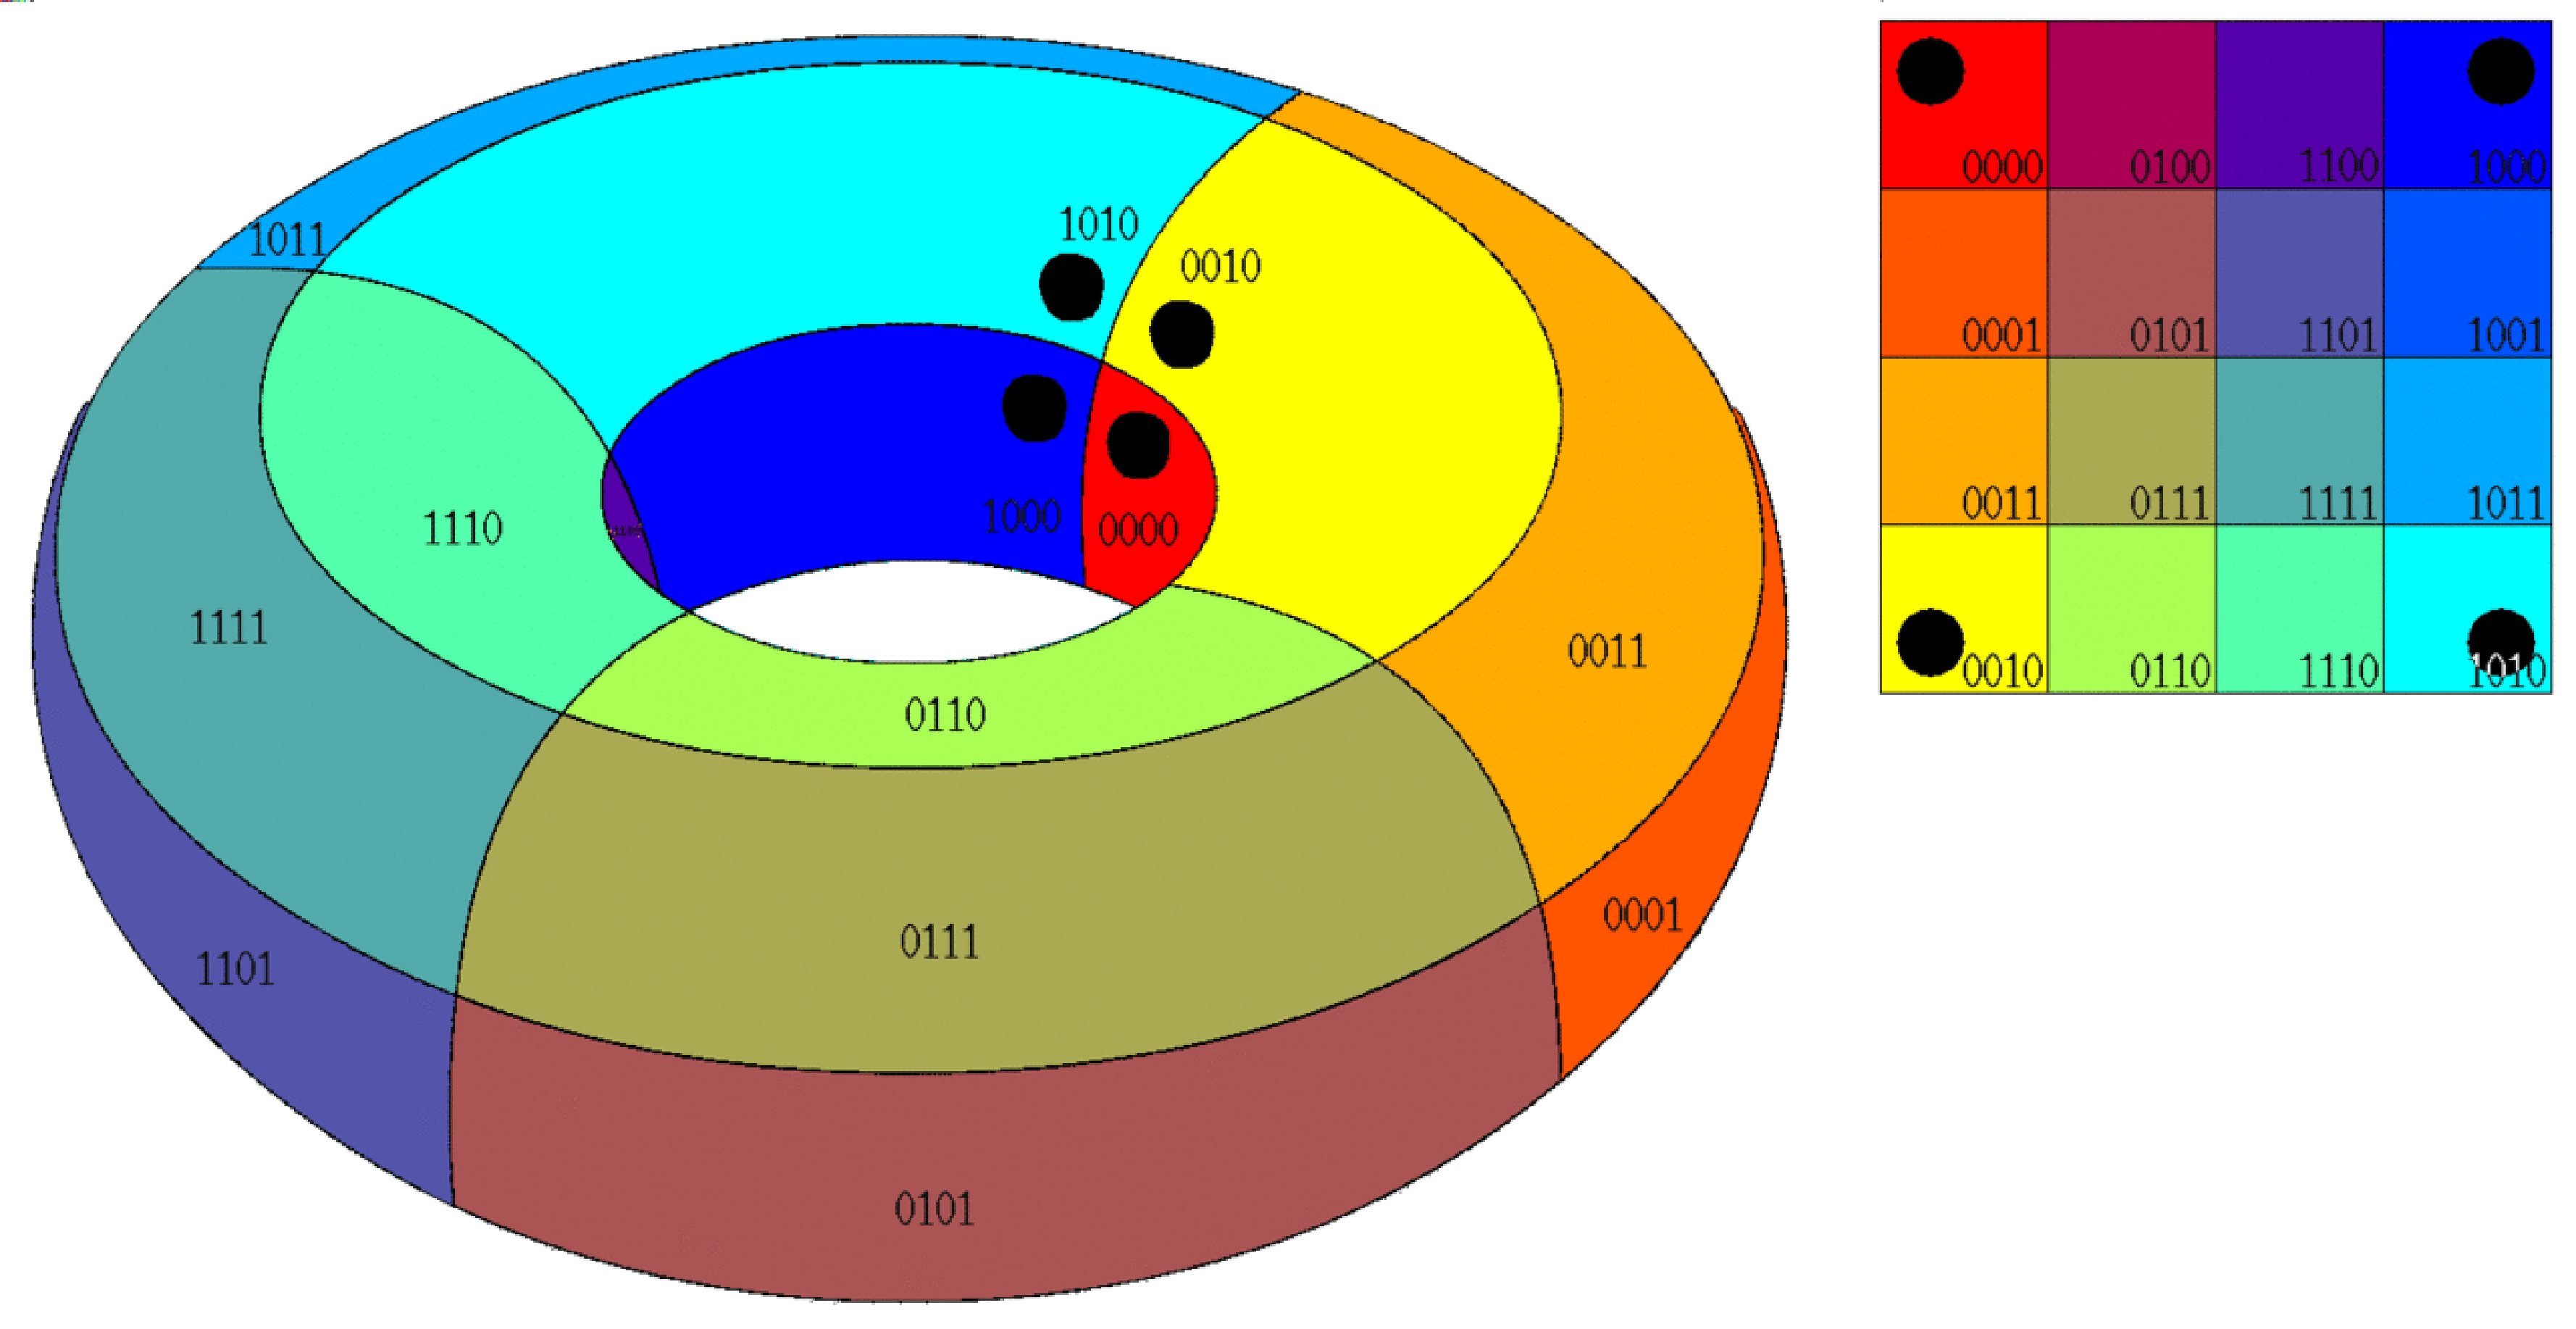
\includegraphics[width=\columnwidth]{Figures/torus.png}

    Na pocetku se upise u svako polje odgovarajuca vrednost funkcije.
    Ako se dve jedinice nalaze jedna pored druge to znaci da se one mogu 
    grupisati, jer se razlikuju samo na jednom mestu.
    Slicno i ako imamo cetiri jedinice koje formiraju pravougaonik.
    Pravila zaokruzivanja:
    \begin{itemize}
        \itemsep0em
        \item Zaokruzuju se samo jedinice.
        \item Svaka jedinica mora da bude zaokruzena bar jednom.
        \item Mogu se zaokruzivati iskljucivo grupa od po $2^k$ polja 
              pravougaonog oblika.
        \item Uvek se zaokruzuju sto vece grupe, cak i ako se tom prilikom 
              neke jedinice ponovo zaokruzuju.
        \item Nakon sto se sve jednice zaokruze, treba proveriti da li je 
              neko od zaokruzivanja postalo suvisno, jer svako njegovo polje 
              pripada i nekom drugom zaokruzivanju.
    \end{itemize}

    Svakom od dobijenih zaokruzivanja odgovara jedna elementarna konjunkcija
    koja sadrzi upravo one literale koju su zajednicik za sva polja koja 
    obuhvata to zaokruzivanje.

    \subsection{Metod Kvin-Meklaskog}

    \begin{enumerate}
        \itemsep0em
        \item Sortiranje savrsenih $\mathcal{KNF}$-ova prema broju ne 
            invertovanih literala.
        \item Grupisanje parova iz susednih klasa (zato sto se razlikuju
            u samo jednom literalu).
        \item Tako grupisani savrseni $\mathcal{KNF}$-ovi se ponovo grupisu
            u sledecoj interaciji. To se ponavlja sve dok je grupisanje 
            moguce.
        \item Sve konjunkcije koje su ostale ne pokrivene nazivaju se 
            \emph{proste implikante}.
        \item Formira se \emph{tabela prostih implikanata}. Kolone su pocetne
            konjunkcije, vrste su proste implikante.
        \item Sa $+$ oznacavamo polje gde proste implikante sadrze pocetne
            konjunkcije.
        \item Oznacavamo bitne pluseve, tj.\ plusevi koji su jedini u svojoj
            koloni.
        \item Drugom oznakom oznacimo pluseve koji se nalaze u istoj
            vrsti kao i bitni plusevi.
        \item Kao rezultat uzimamo samo one vrste koje imaju oznacene pluseve.
    \end{enumerate}

    \emph{Patrikov metod} ima ulogu da pojednostavi drugu fazu u minimizaciji, 
    zato sto je ona eksponencijalne slozenosti za racunar.

    \subsection{Minimizacija u Prisustvu nebitnih vrednosti}

    Karnoove mape: Nebitna vrednost bice tretirana kao 1 ako to polje 
    omogucava vece zaokruzivanje, inace ce biti tretirana kao 0.

    Kvin-Meklaski: Nebitna vrednosti u prvoj fazi se tretiraju kao 1, dok
    se u drugoj fazi tretiraju kao 0.
    
    \section{Logicka Kola}
    
    \emph{Logicko kolo} (eng. \emph{logic circuit}) je uredjaj koji 
    implementira neki skup logickih funkcija u datoj tehnologiji.

    \subsection{Vrednost visoke impedense}
    
    Nekada je moguce da izlaz logickog nema nikakvu vrednost, tj.\ da mu
    izlazna vrednost nije ni 0 ni 1. Tu vrednost nazivamo 
    \emph{vrednost visoke impedense} i obelezavamo je sa $\mathbf{Z}$. Ukoliko
    neki izraz ima vrednost $\mathbf{Z}$, tada taj izraz ne uticne na 
    vrednost ulazna na koji je povezan.

    \subsection{Logicke Kapije}

    \emph{Logicke kapije} ili \emph{gejtovi} su uredjaju koji implementiraju 
    logicke veznika iz izabranog skupa.

    \begin{tabular}{*{3}{c}}
        Naziv kola & Sematska oznaka \\
        \midrule
        buffer  & 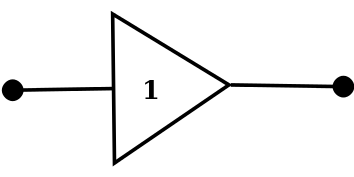
\includegraphics[width=30px]{Figures/buffer.png} \\
        NOT  & 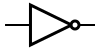
\includegraphics[width=30px]{Figures/not.png} \\
        AND  & 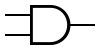
\includegraphics[width=30px]{Figures/and.png} \\
        OR   & 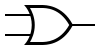
\includegraphics[width=30px]{Figures/or.png} \\
        NAND & 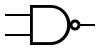
\includegraphics[width=30px]{Figures/nand.png} \\
        NOR  & 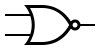
\includegraphics[width=30px]{Figures/nor.png} \\
        XOR  & 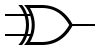
\includegraphics[width=30px]{Figures/xor.png} \\
        XNOR & 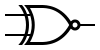
\includegraphics[width=30px]{Figures/xnor.png} \\
    \end{tabular}

    \subsection{Implementacija Logickih Kapija u Savremenim Racunarima}

    Savremeni racunari su zasnivani na jednoj posebnoj vrsti unipolarnih
    tranzistora --- \emph{MOS tranzistori} 
    (eng. \emph{Metal-Oxide-Semiconductor}).
    MOS predstavlja poluprovodnicku komponentu koja ima tri prikljucka:
    \emph{sors} (eng. \emph{source}), \emph{drejn} (eng \emph{drain}), i 
    \emph{gejt} (eng. \emph{gate}).
    MOS tranzistor funkcionise kao prekidac --- struja moze da protice od 
    sorsa ka drajnu po uslovom da se odgovarajuci napon dovede na gejt.
    Kroz gejt ne protice struja vec on stvara elektricno polje kroz koje
    ce struja da tece.
    Postoje dva tipa MOS tranzistora: NMOS i PMOS tranzistor.

    Kod NMOS tranzistora sors mora biti prikljucen na negativan, a drejn na 
    pozitivan napon.
    Da bi doslo do provodjenja struje, potrebno je na gejt dovesti dovoljno 
    veliki pozitivan napon.
    Ukoliko je napon u zoni logicke nule, tada je tranzistor u potpunosti 
    zatvoren i ne provodi struju od sorsa ka drejnu, dok kada je u zoni 
    logicke jedinice od provodi struju.

    Kod PMOS tranzistora sors se prikljucuje na pozitivan, a drajn na 
    negativan napon. 
    Da bi doslo do provodjenja struje, potrebno je na gejt dovesti negativan 
    napon.
    Ukoliko je napon u zoni logicke jedinice, tada je tranzistor u zatvoren i
    ne provodi struju, dok kada je u zoni logicke nule on provodi struju.

    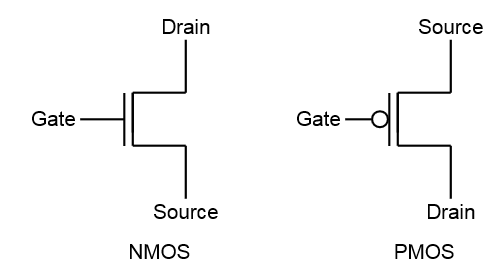
\includegraphics[width=0.8\columnwidth]{Figures/mos.png}

    Ako se u izradi logickig kola koriste i NMOS i PMOS tranzistori, tada
    govorimo o CMOS tehnologiji (eng. \emph{Complementary MOS}).

    \subsubsection{NOT kolo}

    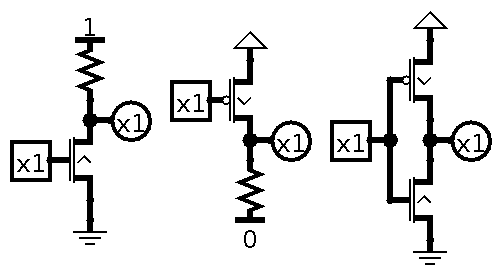
\includegraphics[width=0.7\columnwidth]{Figures/mos_not.png}

    \subsubsection{NAND i AND kolo}

    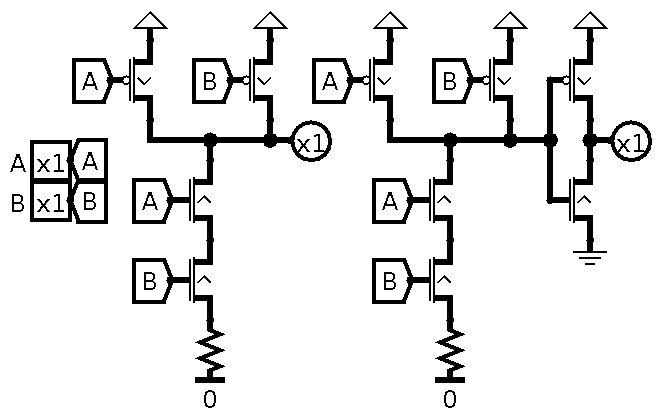
\includegraphics[width=0.8\columnwidth]{Figures/mos_nand_and.png}

    \subsubsection{NOR i OR kolo}

    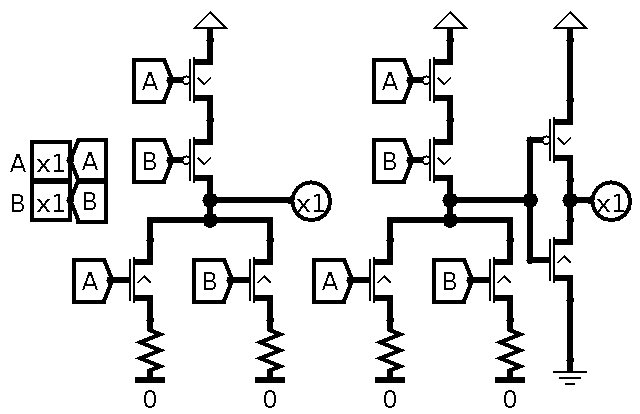
\includegraphics[width=0.8\columnwidth]{Figures/mos_nor_or.png}

    \subsubsection{XOR kolo}

    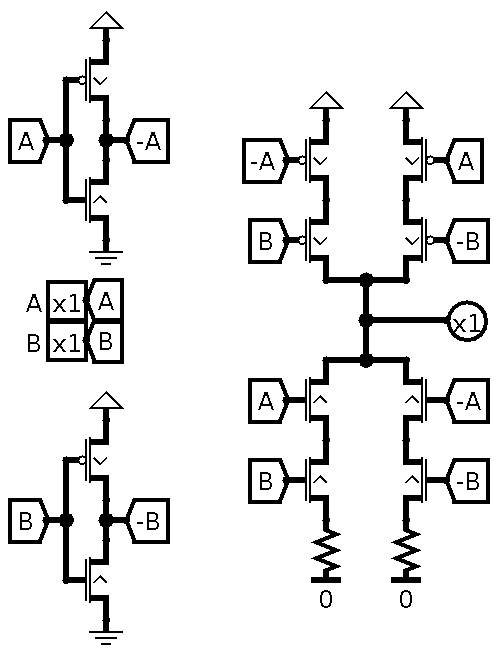
\includegraphics[width=0.7\columnwidth]{Figures/mos_xor.png}

    \subsubsection{Buffer}

    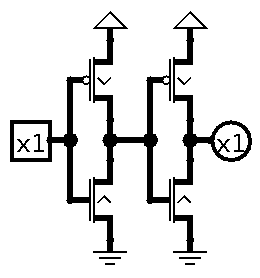
\includegraphics[width=0.4\columnwidth]{Figures/mos_buffer.png}

    \subsubsection{Propusni Tranzistori i Prenosne Kapije}

    \emph{Propusni tranzistori} kontrolisu propustanje nekog signala od jedne 
    tacke kola ka drugoj u zavisnost od vrednosti nekog drugog signala.

    \emph{Propusna kapija} CMOS varijanta propusnih tranzistora.

    \subsection{Baferi sa Tri Stanja}

    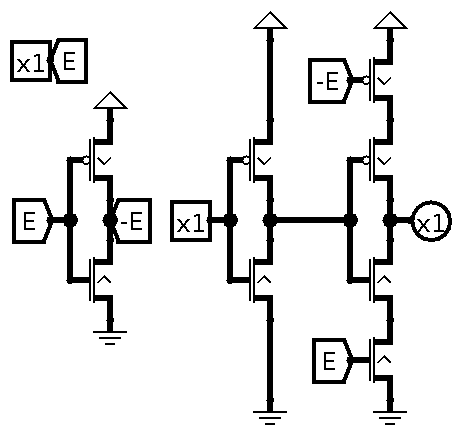
\includegraphics[width=0.7\columnwidth]{Figures/mos_tristate_buffer.png}
    
    \section{Kombinatorna Kola}

    \emph{Kombinatorna kola} (eng. \emph{combinational curcuit}) su kola ko 
    kojih su izlazni signali jednoznacno odredjeni trenutnim ulaznim 
    signalima, tako da predstavljaju jednu logicku funkciju.

    \subsection{Osnovna kombinatorna kola}

    \subsubsection{Multiplekser}

    \emph{Multiplekser} je kolo sa $2^n$ ulaza, jednim izlazom i $n$ 
    upravljackih jedinica pomocu kojih se bira jedna od ulaza koji ce se 
    pojaviti na izlazu.
    
    \paragraph{Primena multipeksera}
    \begin{itemize}
        \itemsep0em
        \item Bira podatak koji se salje na magistralu
        \item Operacija koju ALU mora da izracuna
        \item Dekompozicija logickih funkcija na jendostavnije funkcije
    \end{itemize}
    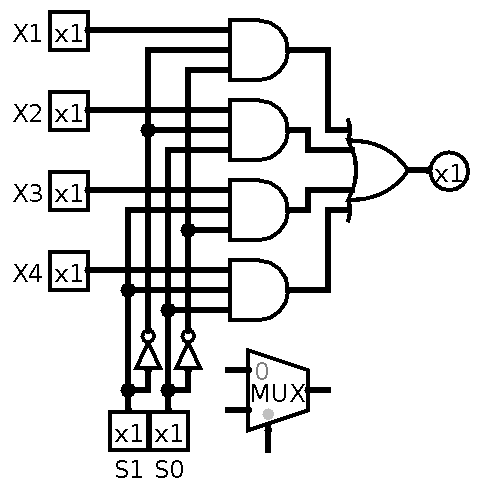
\includegraphics[width=0.7\columnwidth]{Figures/mux.png}

    \begin{tabular}{*{2}{c}}
        $S$ & $f(\mathbf{X}, S)$ \\
        \midrule
        00  & $X_1$ \\
        01  & $X_2$ \\
        10  & $X_3$ \\
        11  & $X_4$ \\
    \end{tabular}

    \subsubsection{Demultiplekser}

    \emph{Demultiplekser} je kolo sa jednim ulazom, $2^n$ izlaza i $n$
    upravljackih jedinica pomocu kojih se ulaz preusmerava na tacno jedan
    izlaz.

    \paragraph{Primena demultipleksera}
    \begin{itemize}
        \itemsep0em
        \item Bira odrediste vrednosti koja se prenosi nekom magistralom
    \end{itemize}
    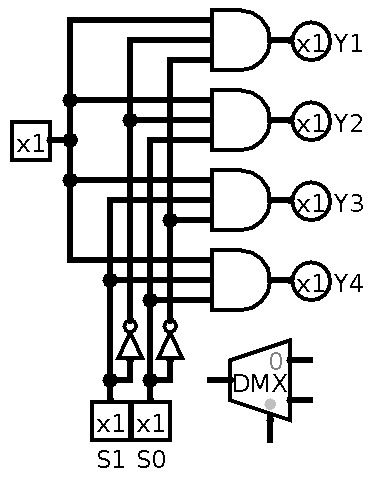
\includegraphics[width=0.6\columnwidth]{Figures/dmx.png}

    \begin{tabular}{*{5}{c}}
        $S$ & $Y_1$ & $Y_2$ & $Y_3$ & $Y_4$ \\
        \midrule
        00  & $x$ &  0  &  0  &  0  \\
        01  &  0  & $x$ &  0  &  0  \\
        10  &  0  &  0  & $x$ &  0  \\
        11  &  0  &  0  &  0  & $x$ \\
    \end{tabular}

    \subsubsection{Dekoder}

    \emph{Dekoder} je kolo koje kao ulazni podatak prihvata $n$-bitni broj, a
    zatim na osnovu njega bira samo jedan on $2^n$ izlaza koji postavlja na 
    vrednost logicke jedinice.

    \paragraph{Primena decodera}
    \begin{itemize}
        \itemsep0em
        \item Odredjuje vrednost broja koji je zadat binarno
        \item Biranje registra iz kog se uzima vrednost
        \item Obrada sistema prekida
    \end{itemize}
    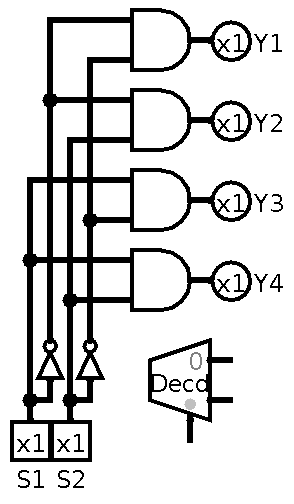
\includegraphics[width=0.4\columnwidth]{Figures/decoder.png}

    \begin{tabular}{*{5}{c}}
        $S$ & $Y_1$ & $Y_2$ & $Y_3$ & $Y_4$ \\
        \midrule
        00 & 1 & 0 & 0 & 0 \\
        01 & 0 & 1 & 0 & 0 \\
        10 & 0 & 0 & 1 & 0 \\
        11 & 0 & 0 & 0 & 1 \\
    \end{tabular}

    \subsubsection{Enkoder}

    \emph{Enkoder} je kolo koje ime $2^n$ ulaza, a zatim na osnovu njih stvara
    $n$-bitni broj.

    \emph{Enkoder sa prijoritetom} sprecava gresku kada se pojave vise od 
    jedne jedinice na ulazu, te on ima prioritet prve jedinice koja se 
    pojavljuje.

    \paragraph{Primene encodera}
    \begin{itemize}
        \itemsep0em
        \item Odredjuje koji od I/O uredjaja trazi prekid
    \end{itemize}
    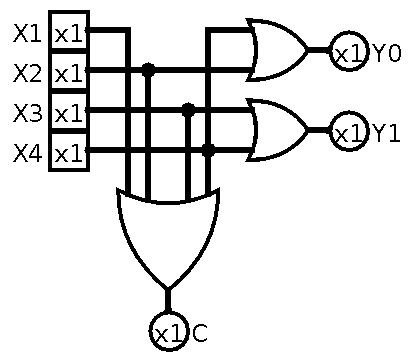
\includegraphics[width=0.6\columnwidth]{Figures/encoder.png}

    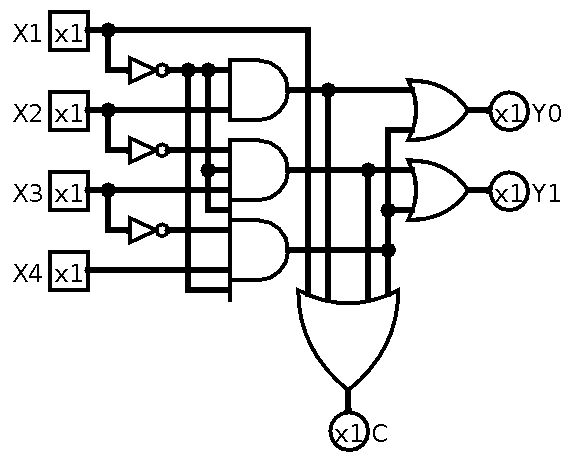
\includegraphics[width=0.8\columnwidth]{Figures/priority_encoder.png}

    \subsubsection{Komparatori}

    \emph{Komparatori} su kola koja porede dve ulazne vrednosti.
    
    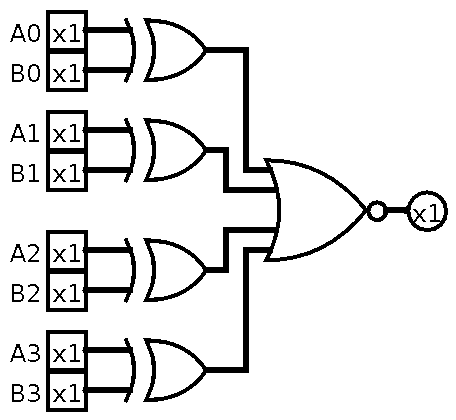
\includegraphics[width=0.6\columnwidth]{Figures/cmp_eq.png}

    \subsection{Aritmeticko-Logicka kola}


    \subsubsection{Pomeraci}

    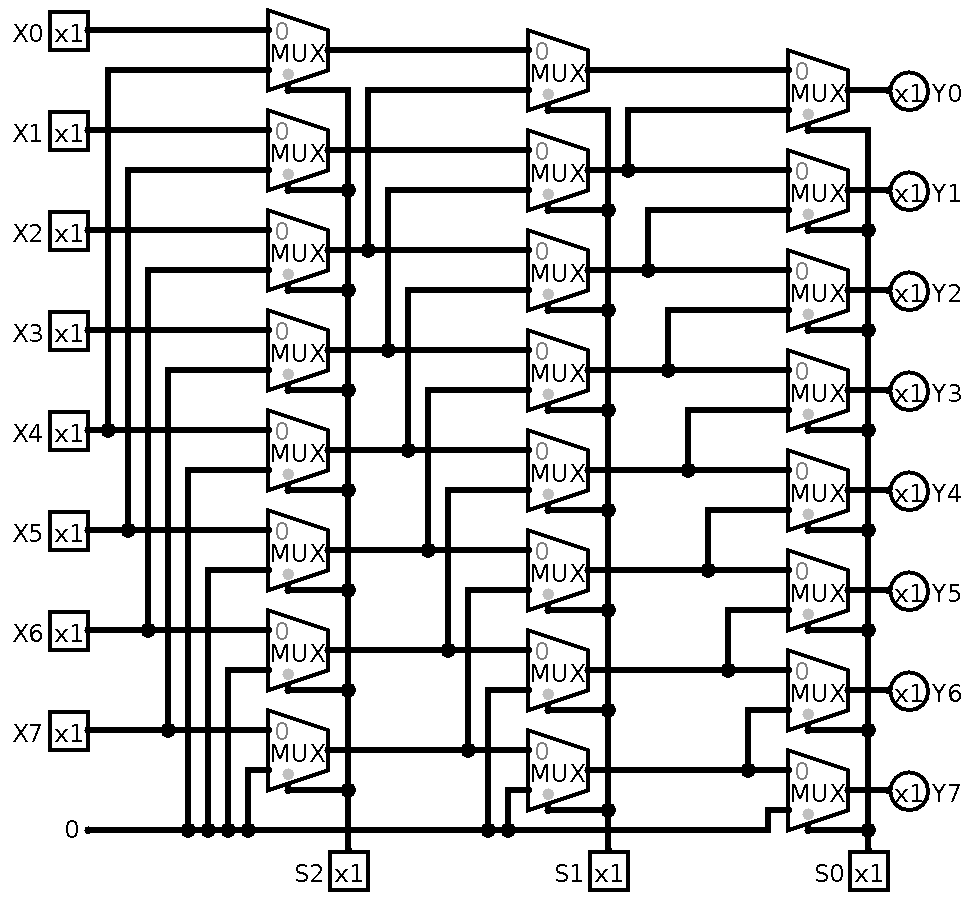
\includegraphics[width=\columnwidth]{Figures/shifter.png}

    \subsubsection{Sabiraci i Oduzimaci}

    \paragraph{Polusabirac}

    \begin{tabular}{*{5}{c}}
        $X$ & $Y$ & $S$ & $C$ \\
        \midrule
         0  &  0  &  0  &  0  \\
         0  &  1  &  1  &  0  \\
         1  &  0  &  1  &  0  \\
         1  &  1  &  0  &  1  \\
    \end{tabular}

    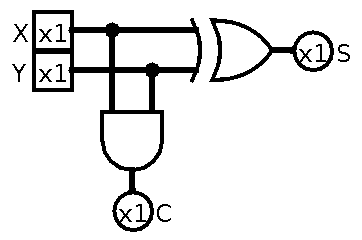
\includegraphics[width=0.5\columnwidth]{Figures/half_adder.png}

    \paragraph{Punisabiraci}

    \begin{tabular}{*{5}{c}}
        $X$ & $Y$ & $PC$ & $S$ & $C$ \\
        \midrule
         0  &  0 &  0  &  0  &  0  \\
         0  &  0 &  1  &  1  &  0  \\
         0  &  1 &  0  &  1  &  0  \\
         0  &  1 &  1  &  0  &  1  \\
         1  &  0 &  0  &  1  &  0  \\
         1  &  0 &  1  &  0  &  1  \\
         1  &  1 &  0  &  0  &  1  \\
         1  &  1 &  1  &  1  &  1  \\
    \end{tabular}

    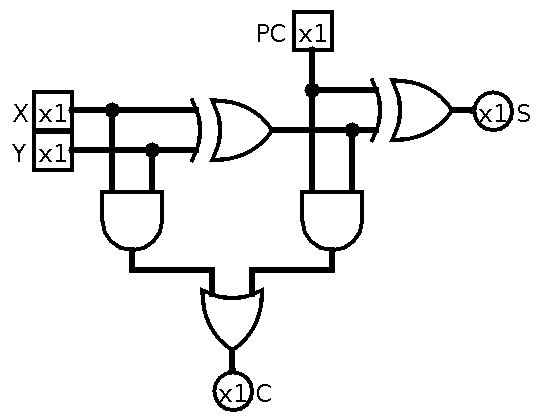
\includegraphics[width=0.7\columnwidth]{Figures/full_adder.png}

    \paragraph{Visebitni sabiraci}
    
    \emph{Visebitni talasasti sabirac} (eng. \emph{Ripple Carry Adder}) je 
    kolo koje je implementirano tako da se za svaki bit pomoci sabiraca 
    racuna zbir i prenos, koji se onda prenosi na sledeci sabirac. Tako 
    ulancani sabiraci, sa po $2\Delta$ kasnjenja, imaju ukupno 
    $n \times 2\Delta$, jer se za svaki prethodni ceka racunanje prenosa. 
    Pr.\ 32-bitni sabirac ima $64\Delta$ kasnjenja.

    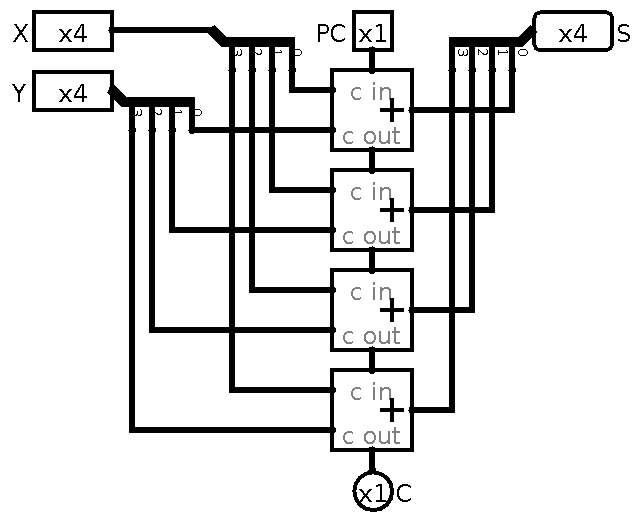
\includegraphics[width=0.7\columnwidth]{Figures/riplle_carry_adder.png}

    \paragraph{Poluoduzimac}
    
    \begin{tabular}{*{4}{c}}
        $X$ & $Y$ & $S$ & $C$ \\
        \midrule
         0  &  0  &  0  &  0  \\
         0  &  1  &  1  &  1  \\
         1  &  0  &  1  &  0  \\
         1  &  1  &  0  &  0  \\
    \end{tabular}

    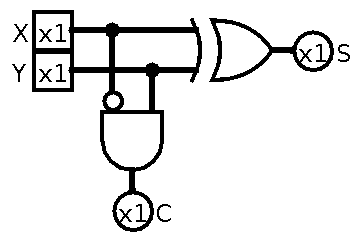
\includegraphics[width=0.5\columnwidth]{Figures/half_sub.png}

    \paragraph{Punioduzimaci}

    \begin{tabular}{*{5}{c}}
        $X$ & $Y$ & $PC$ & $S$ & $C$ \\
        \midrule
         0  &  0 &  0  &  0  &  0  \\
         0  &  0 &  1  &  1  &  1  \\
         0  &  1 &  0  &  1  &  1  \\
         0  &  1 &  1  &  0  &  1  \\
         1  &  0 &  0  &  1  &  0  \\
         1  &  0 &  1  &  0  &  0  \\
         1  &  1 &  0  &  0  &  0  \\
         1  &  1 &  1  &  1  &  1  \\
    
    \end{tabular}

    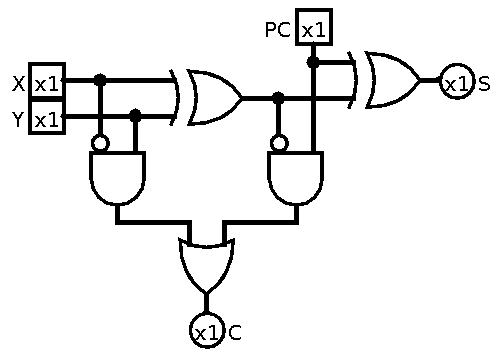
\includegraphics[width=0.7\columnwidth]{Figures/full_sub.png}

    \paragraph{Visebitni oduzimac}

    \emph{Visebitni talasasti oduzimac} (eng. \emph{Ripple Carry Subtractor}) 
    je kolo koje je implementirano tako da se za svaki bit pomoci oduzimaca 
    racuna razliku i prenos, koji se onda prenosi na sledeci oduzimac. Tako 
    ulancani oduzimaci, sa po $2\Delta$ kasnjenja, imaju ukupno 
    $n \times 2\Delta$, jer se za svaki prethodni ceka racunanje prenosa. 
    Pr.\ 32-bitni oduzimac ima $64\Delta$ kasnjenja.

    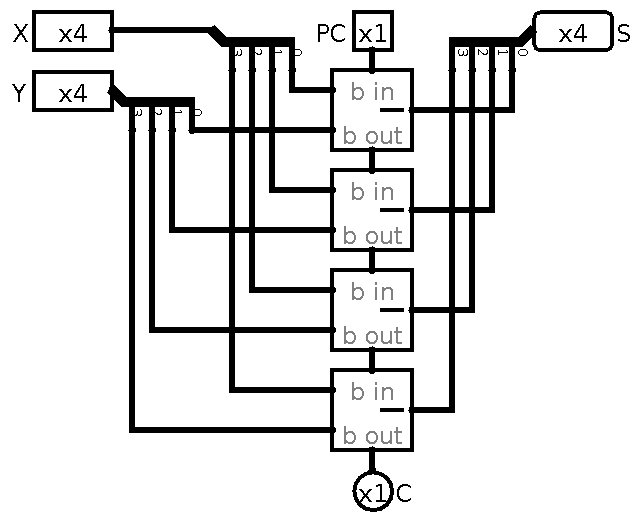
\includegraphics[width=0.7\columnwidth]{Figures/riplle_carry_sub.png}

    \paragraph{Sabirac sa racunanjem prenosa unapred}
    (eng. \emph{Lookahead Carry Adder --- LCA}) racuna prenost unapred kako bi
    se smanjilo kasnjenje visebitnih sabiraca. Neka su $C_i$ prenosi, svakog 
    od $i$ punih sabiraca.
    \begin{align*}
        C_0 &= x_0 y_0 + x_0 pc + y_0 pc \\
        C_1 &= x_1 y_1 + x_1 C_0 + y_1 C_0 \\
            &= x_1 y_1 + x_1 (x_0 y_0 + x_0 pc + y_0 pc) + \\
            &+ y_1 (x_0 y_0 + x_0 pc + y_0 pc)\\
            &= x_1 y_1 + x_1 x_0 y_0 + x_1 x_0 pc + x_1 y_0 pc + \\
            &+ y_1 x_0 y_0 + y_1 x_0 pc + y_1 y_0 pc\\
    \end{align*}

    Ovaj izraz veoma brzo raste tako da nije efikasan.
    \begin{align*}
        C_0 &= x_0 y_0 + x_0 pc + y_0 pc \\
            &= x_0 y_0 + (x_0 + y_0) pc \\
            &= x_0 y_0 + (x_0\oplus y_0) pc \\
            &= G_0 + P_0 pc \\
        C_i &= G_i + P_i C{i-1}, \\
    \end{align*}
    gde je $G_0 = x_i y_i, P_i = x_i \oplus y_i$. Na primer za $C_3$:
    \begin{align*}
        C_1 &= G_1 + P_1 C_0 \\
            &= G_1 + P_1 (G_0 + P_0 pc) \\
            &= G_1 + P_1 G_0 + P_1 P_0 pc \\
        C_2 &= G_2 + P_2 C_1 \\
            &= G_2 + P_2 (G_1 + P_1 G_0 + P_1 P_0 pc) \\
            &= G_2 + P_2 G_1 + P_2 P_1 G_0 + P_2 P_1 P_0 pc \\
        C_3 &= G_3 + P_3 C_2 \\
            &= G_3 + P_3 (G_2 + P_2 G_1 + P_2 P_1 G_0 + P_2 P_1 P_0 pc) \\
            &= G_3 + P_3 G_2 + P_3 P_2 G_1 + P_3 P_2 P_1 G_0 + P_3 P_2 P_1 P_0 pc \\
        C_3 &= G_G + P_G pc, \\
    \end{align*}
    gde je $G_G = G_3 + P_3 G_2 + P_3 P_2 G_1 + P_3 P_2 P_1 G_0$, \\
    $P_G = P_3 P_2 P_1 P_0$.

    \subsubsection{Aritmeticko-Logicka Jedinica}

    \emph{Aritmeticko-Logicka jedinica} 
    (eng. \emph{Arithmetic Logic Unit --- ALU}) je kolo koje izvrsava 
    razlicite aritheticke i logicke operacije, u zavisnosti od zahteva 
    korisnika.

    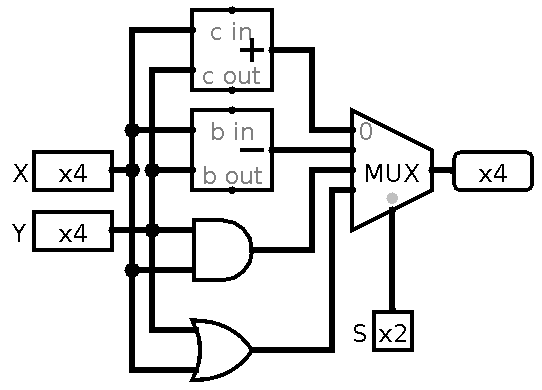
\includegraphics[width=0.6\columnwidth]{Figures/alu.png}

    \subsubsection{Programabilni logicki nizovi}

    \emph{Programabilni logicki nizovi} 
    (eng. \emph{Programmable Logic Array --- PLA}) su programabilna logicka 
    kola koja sluze za implementiranje bilo koje logicke funkcije 
    predstavljene u savrsenom $\mathcal{DNF}$-u.

    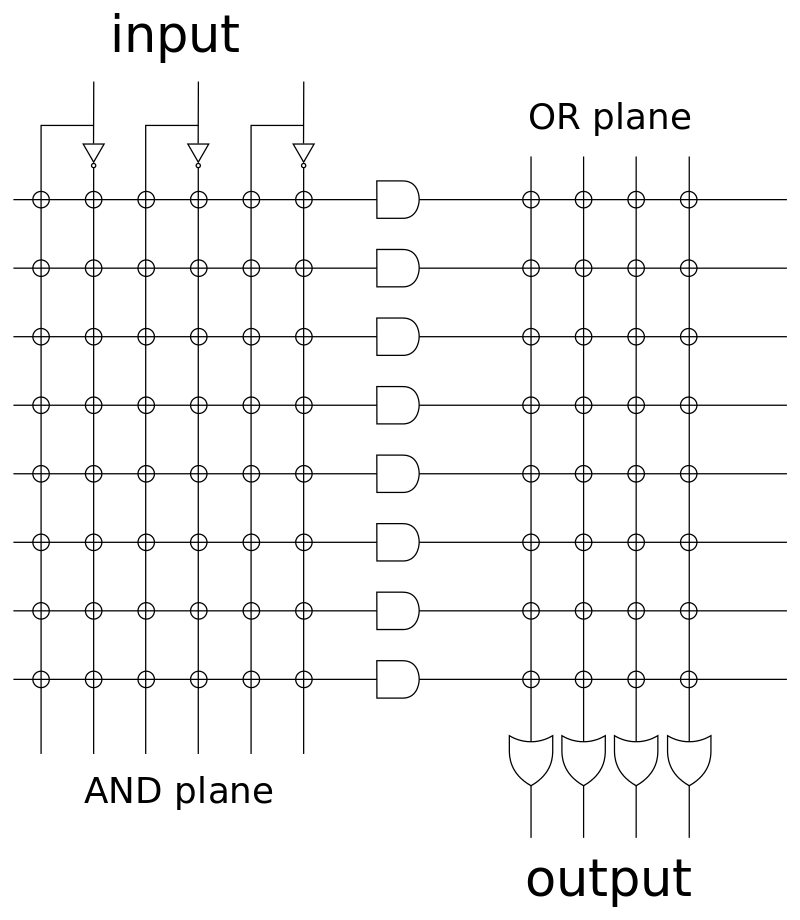
\includegraphics[width=0.8\columnwidth]{Figures/pla.png}

    \subsubsection{ROM}

    \begin{tabular}{*{4}{c}}
        $X_1$ & $X_2$ & $Y_1$ & $Y_2$ \\
        \midrule    
        0 & 0 & 0 & 1 \\
        0 & 1 & 1 & 1 \\
        1 & 0 & 1 & 0 \\
        1 & 1 & 0 & 0 \\
    \end{tabular}

    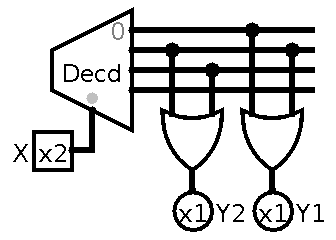
\includegraphics[width=0.5\columnwidth]{Figures/rom.png}

    \section{Sekvencijalna Kola}

    Kod \emph{kombinatornih kola} vrednost na izlazu 
    $\mathbf{Y} = (y_1, y_2, \ldots, y_n)$ u nekom trenutku $t$ vazi 
    iskljucivo od vrednosti na ulazu $\mathbf{X} = (x_1, x_2, \ldots, x_n)$, 
    pa se moze predsaviti kao
    \[
        \mathbf{Y} = F(\mathbf{X}),
    \]
    gde je $F$ neka vektorska logicka funkcija po $\mathbf{X}$.

    Pod \emph{stanjem} podrazumevamo niz bitova 
    $\mathbf{S} = (s_1, s_2, \ldots, s_n)$, koja se pamte unutar kola.
    Da bi se to stanje odrzavalo samo sebe mora da zavisi i od $\mathbf{X}$ i 
    od $\mathbf{S}$:
    \[
        \mathbf{S} = G(\mathbf{X}, \mathbf{S}),
    \]
    gde je $G$ neka vektorska logicka funkcija po $\mathbf{X}$ i $\mathbf{S}$.
    Ovo se realizuje \emph{povratnom spregom}.
    
    \emph{Stabilono stanje} je stanje koje se nece promeniti sve dok se ulaz
    $\mathbf{X}$ funkcije $G$ ne promeni. Dok je \emph{nestabilno stanje}, 
    stanje za koje $\mathbf{S}$ nije fiksirana tacka funkcije $G$.

    \begin{itemize}
        \itemsep0em
        \item Vreme koje je potrebno da se stanje $\mathbf{S}$ stabilizuje u
              stabilno stanje $\mathbf{S'}$ naziva se 
              \emph{vreme stabilizacije}.
        \item Kolo koje osciluje izmedju razlicitih stanja i ne uspeva da 
              dostigne stabilno stanje naziva se \emph{nestabilno}.
        \item Kako kolo koje osciluje izmedju 0 i 1, tj. $+0V$ i $+5V$, u tom
              procesu promene moze da se stabilizuje na $+2.5V$, to stanje
              se naziva \emph{metastabilnost}.
        \item Nekada za dati ulaz $\mathbf{X}$ kolo moze da ode u stabilno 
              stanje $\mathbf{S'}$ ili $\mathbf{S''}$, u zavisnosti od 
              nepredvidljivih fizickih faktora. Ova pojava se naziva 
              \emph{nedeterministicnost}.
    \end{itemize}

    Za kolo kazemo da je \emph{stabilno}, ako za svaku vrednost $\mathbf{X}$ 
    na ulazi i za svako trenutno stanje $\mathbf{S}$ kolo prelazi u stabilno
    stanje $\mathbf{S'}$ koje je jedinstveno odredjeno i zavisi samo od 
    $\mathbf{X}$ i $\mathbf{S}$, tj.\ imamo:
    \[
        \mathbf{S'} = T(\mathbf{X}, \mathbf{S}).
    \]
    Funkcija $T$ naziva se \emph{funkcija prelaska}.

    \subsection{Generatori radnog takta}

    \emph{Radni takt} ili \emph{casovnik} (eng. \emph{clock}) neprekidno 
    emituje impusle odredjene duzine u odredjenim vremenskim razmacima. 

    Prelazak sa 0 na 1 se naziva \emph{ulazna ivica} 
    (eng. \emph{rising edge}).
    Prelazak sa 1 na 0 se naziva \emph{silazna ivica} 
    (eng. \emph{falling edge}).

    Vreme intervala izmedju dve odgovarajuce ivice dva uzastona impulsa 
    naziva se \emph{ciklus radnog takta} (eng. \emph{clock cycle time}).

    Broj ciklusa u sekundi odredjuju \emph{frekvenciju radnog takta}.

    \emph{Sinhroni} radni takt ima jednako trajanje ciklusa, Dok 
    \emph{asinhroni} nema.

    \subsection{Asinhrona i Sinhrona sekvencijalna kola}

    \emph{Asinhrona kola} su sekvencijalna kola kod kojih se menja stanje na
    osnovu izlaza nekog drugog kola.

    \emph{Sinhrona kola} su sekvencijalna kola koja menjaju stanje samo u 
    odredjenom trenutku ciklusa casovnika (uzlazni ili silazni signala).

    Kod sinhronih kola stanje se menja na odredjeno vreme sto je diskretna
    velicina, dok kod asinhronih kola vreme je kontinualna velicina.
    Da bi sinhrona kola radila ciklus radnog takta mora da bude duzi od 
    najveceg kasnjenja nekog kola, sto smanjuje brzinu kola koje imaju malo
    kasnjenje.

    \subsection{Reze}

    \subsubsection{SR reza}

    \emph{SR reza} (eng. \emph{SR latch}) je sekvencijalno kolo koje ima dva
    ulazna bita $S$ (set) i $R$ (reset) i dvobitno stanje $Q\overline{Q}$ 
    koje je ujedno i izlaz i definisano je sa:

    \begin{align*}
        Q &= R \ \NOR\ \overline{Q} \\
        \overline{Q} &= S \ \NOR\ Q 
    \end{align*}.
    \begin{itemize}
        \itemsep0em
        \item $S = 0, R = 0$ reza cuva prethodno stanje
        \item $S = 0, R = 1$ reza resetuje svoje stanje na 0
        \item $S = 1, R = 0$ reza setuje svoje stanje na 1
        \item $S = 1, R = 1$ je nestabilno stanje 
    \end{itemize}

    \begin{tabular}{*{5}{c}}
        $S$ & $R$ & $Q$ & $Q_n$ & Action \\
        \midrule
         0  &  0  &  0  &  0  & hold state\\
         0  &  0  &  1  &  1  & hold state\\
         0  &  1  &  x  &  0  & reset \\
         1  &  0  &  x  &  1  & set \\
         1  &  1  &  x  & --- & not allowed \\
    \end{tabular}

    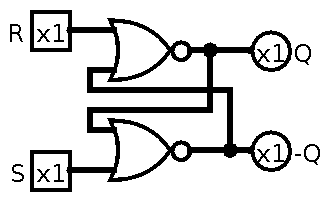
\includegraphics[width=0.5\columnwidth]{Figures/sr_latch.png}

    \subsubsection{D reza}

    \emph{D reza} (eng. \emph{D lathc}) je sekvencijalno kolo, koje za
    razliku od SR reze ima samo jedan ulazni bit $D$ i jedan bit za kontrolu 
    menjanja stanja $e$. Kod D reze nemamo mogucnost nestabilnog stanja, zato
    sto je na $S$ ulazu $D$, a na $R$ ulazu $\overline{D}$. Iz tog razloga
    nikada nije moguce cuvati stanje za bilo koje $D$, pa se uvodi bit za 
    kontrolu stanja $e$, koji menja stanje u zavisnost od $D$ kada je 1, dok
    kada je 0 on cuva stanje. Ukratko vrednost sa $D$ se smesta u D rezu.

    \begin{itemize}
        \itemsep0em
        \item $e = 0$ stanje ostaje isto
        \item $e = 1, D = 0$ stanje se resetuje na 0
        \item $e = 1, D = 1$ stanje se setuje na 1
    \end{itemize}

    \begin{tabular}{*{5}{c}}
        $D$ & $Q$ & $e$ & $Q_n$ & Action \\
        \midrule
         x  &  0  &  0  &  0  & hold state\\
         x  &  1  &  0  &  1  & hold state\\
         0  &  x  &  1  &  0  & reset \\
         1  &  x  &  1  &  1  & set \\
    \end{tabular}

    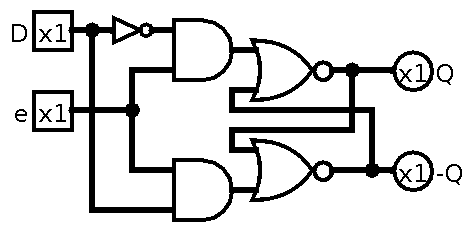
\includegraphics[width=0.7\columnwidth]{Figures/d_latch.png}

    \subsection{Flip-Flop}

    Reze predstavljaju asihnrona sekvencijalna kola. Dok \emph{Flip-Flopovi} 
    predstavljaju najjednostavnija sinhrona kola. Za rad flip-flopova potreban
    je radni takt pa tako oni menjaju svoje stanje samo na ulaznoj/silaznoj
    ivici casovnika.

    \subsubsection{Master-Slave SR flip-flop}

    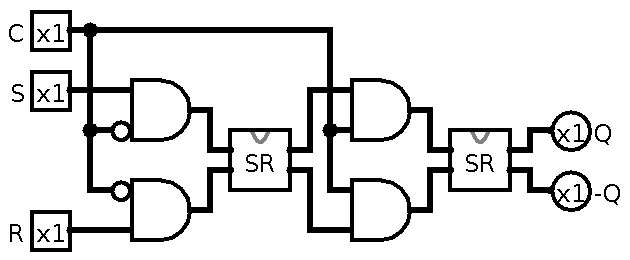
\includegraphics[width=0.8\columnwidth]{Figures/sr_ms_flipflop.png}

    Dok god je signal radnog takta 0, onda se stanje na prvoj SR rezi menja 
    ili ostaje isto u zavisnosti od $S$ i $R$. Kada se signal radnog takta
    promeni na 1, na ulaznoj ivici stanje se menja na drugoj SR rezi, koje
    ujedno i predstavlja stanje SR flip-flopa. Ako se dovedu dve jedinice na
    ulazu dolazi do nestabilnog stanja.

    \subsubsection{Master-Slave D flip-flop}

    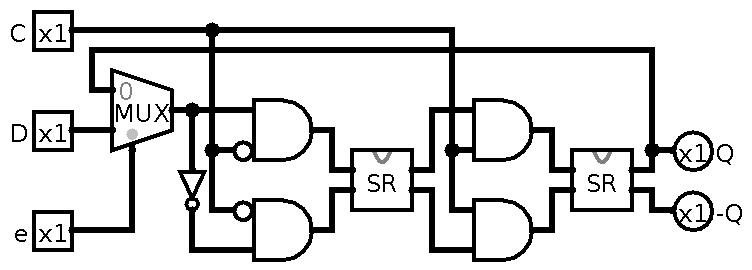
\includegraphics[width=0.9\columnwidth]{Figures/d_ms_flipflop.png}

    Ako je enable bit $e = 0$, stanje se cuva, dok kada je enable bit 
    $e = 1$ stanje prve SR reze postavlja se na vrednost ulaza $D$, kada se
    signal radnog takta promeni sa 0 na 1, stanje se prenosi na drugu SR rezu,
    koje je ujedno i stanje D flip-flopa.

    \subsubsection{Master-Slave JK filp-flop}

    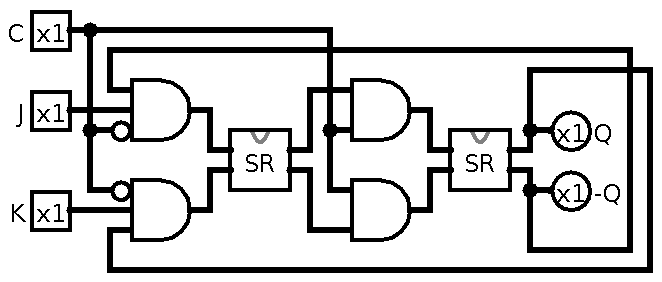
\includegraphics[width=0.9\columnwidth]{Figures/jk_ms_flipflop.png}

    Prva SR reza zavisi od trenutnog stanja JK flip-flopa i ulaza $J, K$. Na
    ulaznoj ivici casovnika stanje sa prve SR reze prebacuje se u drugu sto je
    ujedno i stanje JK flip-flopa.

    \begin{itemize}
        \itemsep0em
        \item $J = 0, K = 0$ stanje ostaje isto
        \item $J = 0, K = 1$ stanje se resetuje na 0
        \item $J = 1, K = 0$ stanje se setuje na 1
        \item $J = 1, K = 1$ stanje prelazi u svoj komplement
    \end{itemize}

    \subsubsection{Master-Slave T flip-flop}

    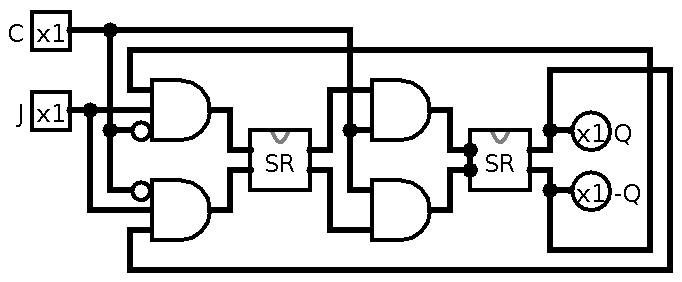
\includegraphics[width=0.9\columnwidth]{Figures/t_ms_flipflop.png}

    Prva SR reza zavisi od trenutnog stanja T flip-flopa i ulaza $T$. Na
    ulaznoj ivica cosovnika stanje sa prve SR reze prebacuje se u drugu sto je
    ujedno i stanje T flip-flopa.

    \begin{itemize}
        \itemsep0em
        \item $T = 0$ stanje ostaje isto
        \item $T = 1$ stanje prelazi u svoj komplement
    \end{itemize}

    \subsubsection{1s Catching Problem}

    \emph{1s catching problem} nastaje kada se na $J$ ili $K$ dovede 1 i pre
    uzlazne ivice casovnika onda vrati na 0. Nakon otkucaja radnog takta 
    stanje JK flip-flopa ce se promeniti u zavisnosti od prethodnog stanja, 
    jer je prva SR reza `uhvatila' tu jedinicu i promenila svoje stanje. 
    Resava se dodavanjem jednog multipleksera koji na ulazu ima 
    $Q, 0, 1, \overline{Q}$, a kontrolni bit mu je 2bitni zapis $JK$.
    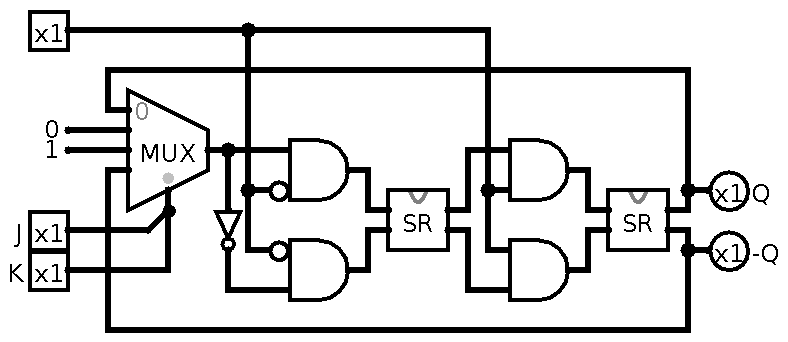
\includegraphics[width=\columnwidth]{Figures/jk_ms_flipflop_1s.png}

    \subsection{Registri}

    \emph{Registar} je kolo koje cuva jedan visebitni binarni broj. Registri
    su napravljeni od jednog niza D flip-flopova, najcesce 8, 16, itd., 
    signalima za citanje i upis.
    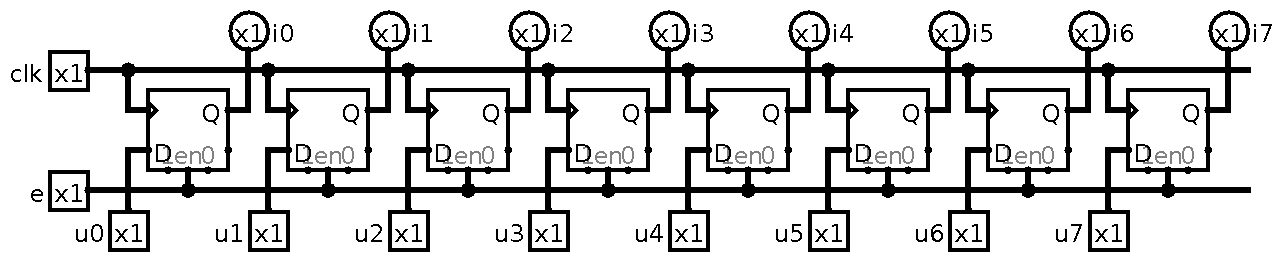
\includegraphics[width=\columnwidth]{Figures/reg_8bit.png}

    \emph{Pomeracki registri} imaju mogucnost pomeranja svog sadrzaja u levo
    ili u desno u svakom ciklusu radnog takta, u zavisnosti od kontrolnih
    signala.
    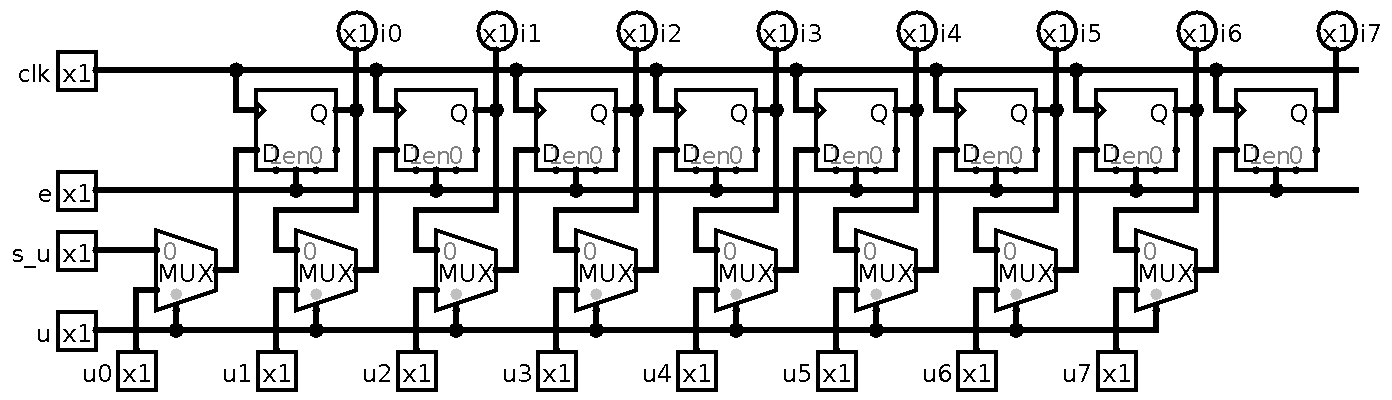
\includegraphics[width=\columnwidth]{Figures/shift_reg.png}

    \subsection{Memorija}
    
    \emph{Staticka memorija} se konstruise pomocu registra koji su 
    hijerarhijski konstruisani pomocu D flip-flopova. Ova memorija je veoma
    brza pa se zato koristi kao kes memorija drugog nivoa.
    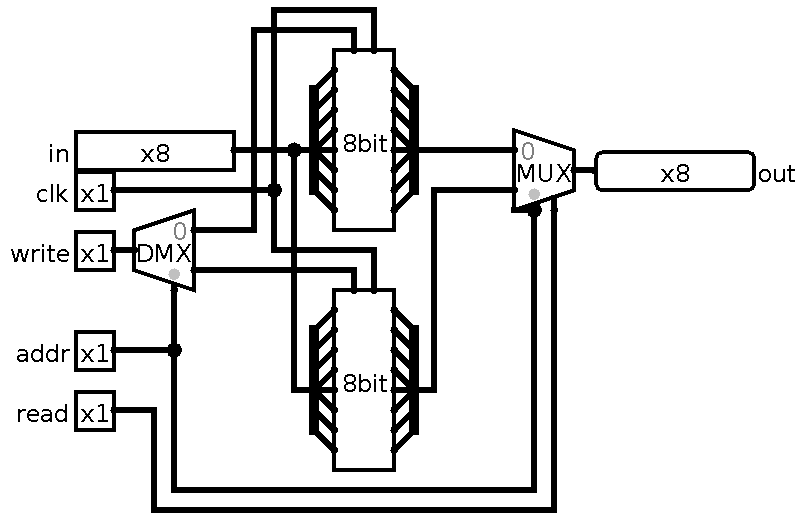
\includegraphics[width=\columnwidth]{Figures/mem28.png}
    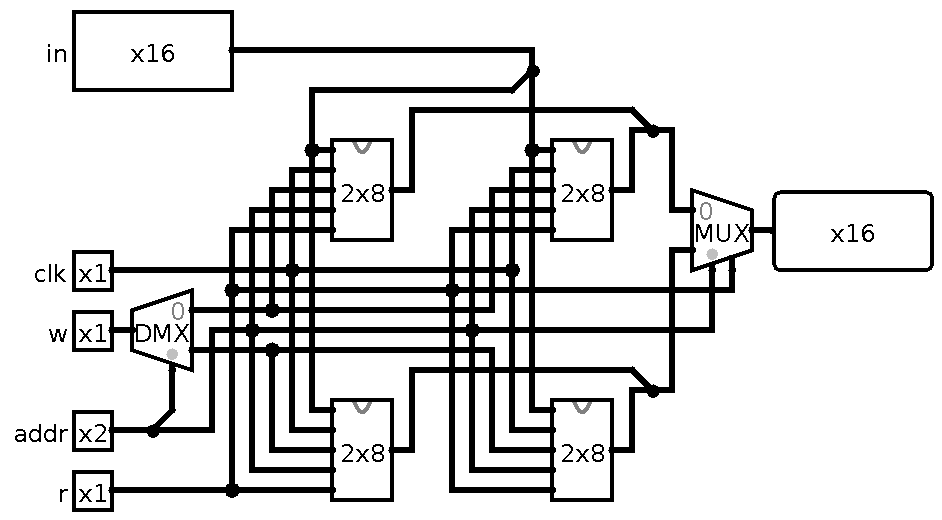
\includegraphics[width=\columnwidth]{Figures/mem416.png}

    \subsection{Brojaci}

    \emph{Asinhroni brojac} radi tako sto stanje na svakog prethodnog kola
    utice na trenutno stanje kolo i tako se prenosi kao talas.

    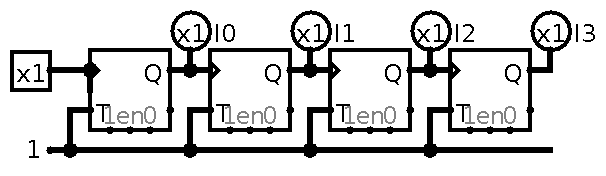
\includegraphics[width=0.8\columnwidth]{Figures/asinhroni.png}

    \emph{Sinhroni brojac} radi tako sto stanje na svim kolima utice od 
    predhodnih stanja i menja se na svakom otkucaju casovnika.

    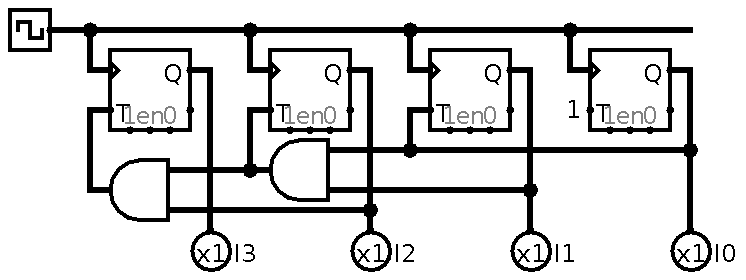
\includegraphics[width=0.9\columnwidth]{Figures/sinhroni.png}

    \emph{Sinhroni brojaci sa proizvoljnim redosledom stanja} se dizajniraju
    tako sto se:    
    \begin{enumerate}
        \itemsep0em
        \item Pravi se tablica ekscitacije stanja
        \item Minimizacija svakog od ulaza $J_i K_i$
        \item Implementacija na osnovu te minimizacije
    \end{enumerate}

    \subsection{Automat i Transdruktor}

    \emph{Koncani automat} je sekvencijalno kolo koje u zavisnost od ulaza i
    trenutnog stanja prelazi u zeljeno stanje. Ako on tada generise i neki
    izlaz, tada ga zovemo \emph{konacnim transduktorom}. 

    Konacni trasnduktor je najopstiji model sinhronog sekvencijalnog kola.
    Pomocu njega se prave kontrolne jedinice u procesoru.

    Implementacija konacnih automata i transduktora je slicna implementacija 
    brojaca sa proizvoljnim redosledom stanja, jedino sto sada na sledece
    stanje uticu i bitova na ulazi.

    \section{Procesorska Organizacija i Performanse}

    \subsection{Datapath}
        
    \emph{Putanja podataka} (eng. \emph{datapath}) je skup funkcionalnih 
    jedinica kao sto je aritmeticko-logicka jedinica, registra, i magistrala.

    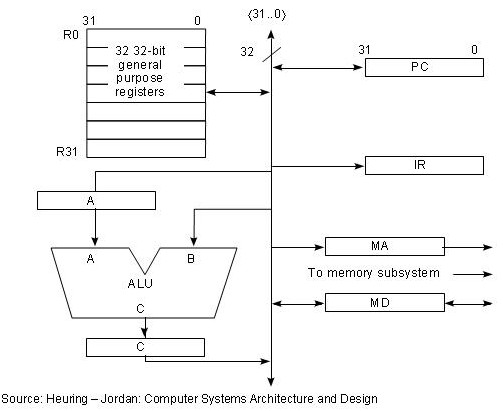
\includegraphics[width=\columnwidth]{Figures/1bus_datapath.jpg}

    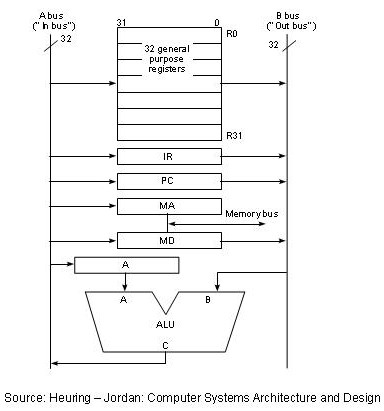
\includegraphics[width=\columnwidth]{Figures/2bus_datapath.jpg}

    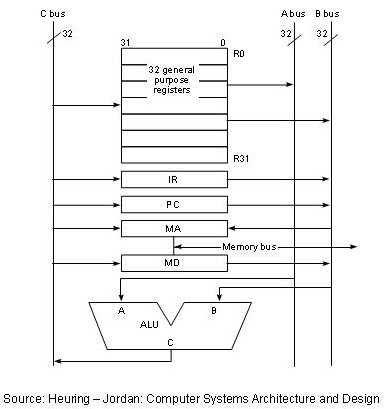
\includegraphics[width=\columnwidth]{Figures/3bus_datapath.jpg}

    \subsection{Kontrolna Jedinica}

    \emph{Kontrolna jedinica} (eng. \emph{Control Unit --- CU}) je kolo
    koje upravlja svim komponentama procesora. Onda u svakom ciklusu 
    casovnika generise \emph{kontrolne signala} koji svim komponentima
    govore sta treba da rede u tom koraku. Primer kontrolnih signala koje
    CU generise su:
    \begin{itemize}
        \itemsep0em
        \item \texttt{reg\_adr}: signal koji selektuje registar iz koga se 
            vrsi citanje ili u koji se vrsi upisivanje
        \item \texttt{reg\_in}: signal koji zahteva od izabranog registra da 
            prihvati i sacuva vrednost sa magistrale
        \item \texttt{reg\_out}: signal koji zahteva da izabranog registra da 
            svoju vrednost poslaje na magistralu
        \item \texttt{p\_in}: signal koji zahteva od P registra da prihvati
            i sacuva vrednost sa magistrale
        \item \texttt{alu\_op}: signal koji selektuje operaciju koju treba da
            izvrsi ALU jedinica
        \item \texttt{psw\_in}: signal koji zahteva od PSW registra da sacuva
            izracunate flegove iz ALU jedinice
        \item \texttt{a\_in}: signal koji zahteva od A registra da sacuva
            izracunatu vrednost sa ALU jedinice
        \item \texttt{a\_out}: signal koji zahteva od A registra da svoju 
            vrednost posalje na magistralu
    \end{itemize}

    Registri reaguju na ulazni rub casovnika, dok kontrolna jedinica salje
    signale na silaznom rubu casovnika, kako bi kontrolna jedinica imala vreme
    da u obzir uzme vrednost flegova u PSW registru pri razunanju novog 
    stanja.

    Kontrolna jedinica je jedan konacni transduktor koji na ulazu ima 
    vrednost PSW registra, a na izlazu ima kontrolne signale. Stanja konacnog 
    transduktora odgovaraju pozicijama u algoritmu koji se izvrsava.

    Svaki algoritam se moze predstaviti kao niz ovih elementarnih koraka.
    
    \begin{itemize}
        \itemsep0em
        \item Naredba dodele: $R_i = R_j$
            \begin{enumerate}
                \itemsep0em
                \item $R_j \texttt{ no\_op1 } P \rightarrow A, PSW$
                \item $A \rightarrow R_i$
            \end{enumerate}
        \item Naredba zbira: $R_i = R_j + R_k$
            \begin{enumerate}
                \itemsep0em
                \item $R_k \rightarrow P$
                \item $R_j \texttt{ add } P \rightarrow A, PSW$
                \item $A \rightarrow R_i$
            \end{enumerate}
        \item Uperedjivanje: $R_i < R_j$
            \begin{enumerate}
                \itemsep0em
                \item $R_j \texttt{ sub } P \rightarrow A, PSW$
                \item $A \rightarrow R_i$
            \end{enumerate}
        \item Negacija: $R_i = -R_j$
            \begin{enumerate}
                \itemsep0em
                \item $R_J \texttt{ neg } P \rightarrow A, PSW$
                \item $A \rightarrow R_i$
            \end{enumerate}
    \end{itemize}

    Primer:
    \begin{lstlisting}
        if (R0 > R1) R2 = R1
        else R2 = R0
    \end{lstlisting}

    \begin{enumerate}
        \itemsep0em
        \item [0.] $R_0 \rightarrow P \ (1)$
        \item [1.] $R_1 \texttt{ sub } P \rightarrow A, PSW \ (2)$
        \item [2.] $C \texttt{ == } 1 \texttt{ ? } R1 \texttt{ no\_op1 } 
            P \rightarrow A, PSW \ (3)$
        \item [2.] $C \texttt{ != } 1 \texttt{ ? } R0 \texttt{ no\_op1 } 
            P \rightarrow A, PSW \ (3)$
        \item [3.] $A \rightarrow R_2 \ (4)$
        \item [4.] --- \ $(4)$
    \end{enumerate}

\end{multicols}

\end{document}
